\documentclass{article}

\usepackage{ctex}
\usepackage{tikz}
\usetikzlibrary{cd}

\usepackage{amsthm}
\usepackage{amsmath}
\usepackage{amssymb}

\usepackage{unicode-math}


\usepackage[textwidth=18cm]{geometry} % 设置页宽=18

\usepackage{blindtext}
\usepackage{bm}
\parindent=0pt
\setlength{\parindent}{2em} 
\usepackage{indentfirst}

\usepackage{graphicx} %图片

\usepackage{xcolor}
\usepackage{titlesec}
\titleformat{\section}[block]{\color{blue}\Large\bfseries\filcenter}{}{1em}{}
\titleformat{\subsection}[hang]{\color{red}\bfseries}{}{0em}{}
%\setcounter{secnumdepth}{1} %section 序号

\newtheorem{theorem}{Theorem}[section]
\newtheorem{lemma}[theorem]{Lemma}
\newtheorem{corollary}[theorem]{Corollary}
\newtheorem{proposition}[theorem]{Proposition}
\newtheorem{example}[theorem]{Example}
\newtheorem{definition}[theorem]{Definition}
\newtheorem{remark}[theorem]{Remark}
\newtheorem{exercise}{Exercise}[section]

\newcommand*{\xfunc}[4]{{#2}\colon{#3}{#1}{#4}}
\newcommand*{\func}[3]{\xfunc{\to}{#1}{#2}{#3}}

\begin{document}
\title{Topology}
\author{枫聆}
\maketitle

\tableofcontents
\section{写在最前面}

拓扑对我来说是新名字,我对它几乎一无所知,虽然我嘴上总是吵吵着代数拓扑是我的终极目标\verb|(~ o ~)~zZ|,终于今天抱着巨大的勇气翻开了包志强老师的《点集拓扑和代数拓扑引论》,被文中老师幽默的行文,深深折服了,似乎拓扑也并没有想象中那么难,我想这是还不错的开始,我的第一直观感受拓扑也是给定一堆对象,在上面用一些公理弄些不一样的结构,似乎和代数一样,但是我暂时还不知道这堆结构要拿来干什么?有什么有趣的性质?

好吧,前面的路还很长,路漫漫,不过一想到前路那些绮丽的景色,多少还是有些兴奋的!虽然这路上没有一起分享喜悦的人...

2020年11月29日23:12:17

\section{Topology Space}
\subsection{Definition of Topology Space} 
预备知识

\begin{itemize}
	\item 对于开集$U$%的理解,首先它是$X$的子集,并且对于$\forall x \in U$,存在$x$的邻域包含于$U$。包老师的书里解释为$U$是每一个$x$的邻域,我感觉在这里似乎有点强了。wiki上解释为实数轴上的开区间的一般性推广。
	\item 子集族是指$X$幂集的子集,所有子集族构成的集合则是$2^{(2^X)}$				
\end{itemize}


拓扑定义的直觉来自于微积分中连续函数的"$\varepsilon-\delta$"语言定义。

\begin{definition}
如果函数$\func{f}{\mathbb{R}}{\mathbb{R}}$满足: 任取$\varepsilon > 0$,存在$\delta > 0$使得$|x-x_0| < \delta$,对$|f(x)-f(x_0)| < \varepsilon$成立。
\end{definition}

这个定义需要$|x-x_0| < \delta$和$|f(x)-f(x_0)| < \varepsilon$这样的度量关系来定义,但是对于抽象的结构,不需要这样具体的度量关系,所以我们抽象的“邻域”来描述两点之前的具体,把所有接近$x_0$程度为$\delta$的点记做$B_{\delta}(x_0)$,这就是邻域的形式化表示,然后对于各种稀奇古怪的接近标准都可以用这个形式来表示。于是乎上面的连续定义可以稍微变一下了

\begin{proposition}
如果函数$\func{f}{\mathbb{R}}{\mathbb{R}}$满足对任意的$\varepsilon > 0$,存在$\delta > 0$有$x \in B_{\delta}(x_0)$,使得$f(x) \in B_{\varepsilon}(f(x_0))$,即$B_{\delta}(x_0) \subseteq f^{-1}(B_{\varepsilon}(f(x_0)))$
\end{proposition}

完美的略掉了度量关系,在这里$B_{\delta}(x_0)$表示$\{x \in \mathbb{R} |\ |x-x_0| < \delta \}$,最后那个包含关系是指$f(x_0)$的任何$\varepsilon$程度下的原像包含$x_0$的某个$\delta$邻域.

是否我们可以通过上面这种定义邻域的方式去把度量空间变成一般拓扑空间呢?当然是可以的,但是我们现在还没有给出邻域的一般定义。那邻域是什么?在邻域之前,应该先理解基准开邻域结构(base open neighborhood),像定义代数结构一样,基准开邻域结构是一个映射(算子)$\func{\mathcal{N}}{X}{2^(2^X)}$,把每一个点$x \in X$对应到一个子集族$\mathcal{N}(x)$上,满足下面几条公理
		\begin{itemize}
			\item $\forall x \in X,\mathcal{N}(x) \neq \emptyset,$并且$\forall U \in \mathcal{N}(x),x \in U$
			\item 若$U,V \in \mathcal{N}(x),$则存在$W \in \mathcal{N}(x)$,使得$W = U \cap V$
			\item 若$y \in U \in \mathcal{N}(x)$,则存在$V \in \mathcal{N}(y)$,使得$V \subseteq U$
		\end{itemize}
用文字来叙述就是
		\begin{itemize}
			\item 每一个$x$都一定有基准开邻域,并且是其任意基准开邻域的元素
			\item $x$的任意两个基准开邻域的交是$x$的邻域
			\item 任意基准开邻域是其所含每个元素$y$的邻域
		\end{itemize}
如果$U$是$x$的一个邻域,则$U$包含了某个$x$基准开邻域,在这里其实我们又可以在基准开邻域的基础上,把邻域也公理化,需要加上一个公理,如果$U$是$x$的一个领域,则$U$的任意超集也是$x$的一个邻域。

我们现在可以用邻域的公理来定义拓扑空间,用$\mathbf{N}$表示一个邻域拓扑,即$\mathbf{N}$表示一个所有非空的$\mathbf{N}(x)$构成的邻域族,最后$(X,\mathbf{N})$表示一个拓扑空间,这种构造方式是Hausdorff提出来的,但是一般地经常用开集的公理来定义领域。

用$(X,\uptau)$表示一个拓扑空间,其中$\uptau$表示$X$的一个子集族,并且满足下面公理:
\begin{itemize}
	\item $\emptyset \in \uptau,X \in \uptau$
	\item $\uptau$中任意两个元素的交集仍属于$\uptau$
	\item $\uptau$中任意多个元素的并集仍属于$\uptau$
\end{itemize}	
则称$\uptau$里面的元素为开集,$\uptau$表示$X$上的一个拓扑结构

开集定义的拓扑空间看起来要比邻域定义,要稍微简洁那么一点,两个定义都是等价的,你可以用邻域的推到开集。在邻域上基础上我们定义如果$U$是$X$的一个子集,且$U$是每一个$x \in U$的领域,则称$U$是一开集。基准开邻域的第三条公理告诉我们基准开邻域肯定是一个开集,然后我们给出一个命题

\begin{proposition}
一个集合是开集当且仅当它是若干个基准开领域的并集
\end{proposition}

\begin{proof}
如果当一个集合是开集时,根据开集的定义,它里面每个元素都有一个邻域,而每个邻域至少包含一个基准开邻域,因此所有基准开邻域的并构成了这个开集。反之若干个基准开领域的并,还是一个基准开领域,前面说过基准开领域是一个开集。

注意,空集也是一族基准开领域的并,只不过这个集合族是空族。
\end{proof}

这个命题证明以后,现在来看看我们用邻域定义得到的开集是否遵循开集的基本公理?很显然地,当并集是基准开领域并的情况下,是满足上诉的开集公理的。回顾前面的定义,基准开邻域在这里起了不小作用,那为什么不一开始使用基准开邻域来定义开集呢?而是使用邻域?下面引用一段包老师的话,写的真好!

基准开邻域结构(三条公理)和邻域结构(四条公理)都能刻画连续性。通常邻域结构很多,并不方便写出来,而基准邻域结构则是比较容易写出的,但它的缺点是:同一种连续性可以用不同的基准开邻域来描述。打个比方,邻域结构就是一个线性空间里面所有的向量,而基准开邻域相对于一个线性空间里面的基,所以很显然,在定义拓扑概念时,我们是希望从具有确定性的邻域结构出发去定义,等到具体计算的时候再用基准开邻域,而不是从基准开邻域结构出发去写一个表达式,用不那么确定的公式作为定义。当然邻域结构里面仍然包含很多冗余信息,因此我们最终选择另一套与之相互唯一确定的,更加简洁齐整的东西,把它称为拓扑结构(开集族)

当我们把一个拓扑空间当一个整体去研究的时候,用开集公理要比邻域的公理更加方便,领域公理似乎更强调“$x$点附近”会怎么样了?但是开集要更抽象一点,需要花些时间去理解,好吧我已经花了不少时间了!!!

\begin{example}
集合$X$上的一个平凡拓扑为$\{X,\emptyset\}$,形象一点说就是“在$X$上无论怎么着都算充分接近”,即取一个$X$作为$x$的基准开邻域,平凡拓扑是$X$上最小的拓扑结构。
\end{example}

\begin{example}
集合$X$上的一个离散拓扑为$\{X,2^{X}\}$,形象一点说就是“在$X$上只有等于$x$才算是和$x$充分接近”,离散拓扑是$X$上最大的拓扑结构。 暂时不理解为什么是等于,而不是包含,但是最大的子集族确实是$2^{X}$
\end{example}

%https://math.stackexchange.com/questions/157735/definition-of-neighborhood-and-open-set-in-topology
\subsection{Properties of Topology Space}

一般的基本定义都会从开集出发,如何从开集出发去定义邻域呢?

\begin{proposition}
一个子集$A$是$x$的邻域当且仅当存在开集$U$,使得$x \in U \subseteq A$.
\end{proposition}

\begin{proof}
只需要证明这样定义出来的邻域是满足上面那4条公理的就行,除了第三条其他的都比较显然,怎么证明第三条呢?$U$是一个开集,$U$自己包含自己,任意$x \in U$,根据开集给出的邻域定义,$U$是$x$的邻域,这样第三条我们也证明了,哈哈,包老师在这里的证明似乎循环论证了lol
\end{proof}


\begin{definition}
如果$A$是$x$的邻域,则称$x$为$A$的\textbf{内点}(interior point).全体内点构成的集合称为\textbf{内部}(interior point),记做$A^{\circ}$
\end{definition}

内点和内部的概念,需要建立在具体的拓扑结构上,取不同的拓扑结构会得到完全不同的结论。

\begin{center}
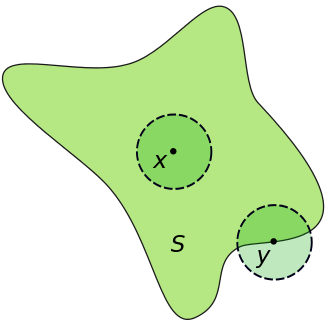
\includegraphics[width=5cm, height=4cm]{images/Interior_illustration.png}
\end{center}



\begin{proposition}
集合的内部具有以下基本性质:
\begin{itemize}
	\item $A^{\circ}=A$当且仅当$A$是开集;
	\item $A^{\circ}$是$A$包含的所有开集的并集,也是$A$中最大的开集;
	\item 若$A \subseteq B$,则$A^{\circ} \subseteq B^{\circ}$;
	\item $(A_1 \cap \ldots \cap A_n)^{\circ}=A_1^{\circ} \cap \ldots \cap A_n^{\circ}$;
	\item ${\left(\bigcup\limits_{i \in n} A_i\right)}^{\circ} \supseteq \bigcup\limits_{i \in n} A_i^{\circ}$
\end{itemize}
\end{proposition}
\begin{proof}
\begin{enumerate}
	\item 这个性质根据开集的定义很显然。
	\item 如果$A$的子集是一个开集,这个子集很显然也是属于$A^{\circ}$,所以$A$里面的所有开集含于$A^{\circ}$,如何证明$A^{\circ}$是一个开集呢?任取$A^{\circ}$中一点$x$,$A$是x的邻域,那么一定存在一个包含$x$的基准开邻域,我们最大基准开邻域是一个并集,根据基准开邻域的定义,这个基准邻域肯定也是属于$A^{\circ}$,所以$A^{\circ}$是其每个点$x$的邻域,所以$A^{\circ}$是一个开集,同时也证明了它是所有这样点$x$的基准开邻域的并。再来证明它是$A$内最大的开集,假设如果它不是$A$内最大的开集,那么存在$A^{'}$包含$A^{\circ}$,但是呢$A'$是其所有点的邻域(根据开集定义),所有$A'$属于$A^{\circ}$,这样产生了矛盾,所以$A^{\circ}$是最大的开集。
	\item 根据邻域的最后一条公理,邻域的超集还是邻域,所以B是$A^{\circ}$中所有点的邻域,所以很自然的$A^{\circ} \subseteq B^{\circ}$
	\item 等式的左边表示,所有集合的交的内部,等式的右边表示,所有集合的内部的交,这里为什么等价呢?这个关系用图来说是非常明显的,怎么用文字呢?应该用数学归纳法来证明,我先证明对两个集合是成立的,首先利用第2个性质,${(A_1 \cap A_2)}^{\circ}=U_1 \cup \ldots \cup U_n $,其中$U_1,\ldots,U_n \in A_1 \cap A_2$,很显然它们也属于$A_1^{\circ}$和$A_2^{\circ}$,即${(A_1 \cap A_2)}^{\circ} \subseteq A_1^{\circ} \cap A_2^{\circ}$,反过来$A_1^{\circ} \cap A_2^{\circ}$是一个开集,并且属于$(A_1 \cap A_2)$,所以$A_1^{\circ} \cap A_2^{\circ} \subseteq {(A_1 \cap A_2)}^{\circ}$,两边一夹所以,${(A_1 \cap A_2)}^{\circ} = A_1^{\circ} \cap A_2^{\circ}$,再用一下数学归纳法,即可。
	\item 这个也需要数学归纳法来证明,这里只证明两个集合的情况下,$A_1^{\circ} \cup A_2^{\circ} \subseteq {(A_1 \cup A_2)}^{\circ}$这还是显然的,用第三条性质就可以知道。但是反过来不一样成立,$A_1$和$A_2$的"公共边界"上的点,完全有可能变成$A_1 \cup A_2$内部的点。
	\begin{center}
		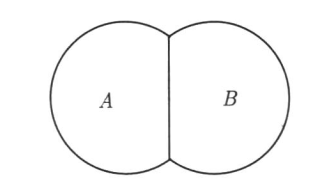
\includegraphics[width=4cm, height=2cm]{images/A_B_same_border.png}
	\end{center}	
\end{enumerate}
\end{proof}

\begin{definition}
如果在拓扑空间$(X,\tau)$中,子集$A$的余集$A^{c}$是开集,则称$A$为\textbf{闭集}(closed set)
\end{definition}

其中余集$A^{c}= X \smallsetminus A$,在平凡拓扑中,闭集就是$\emptyset$和$X$;在离散拓扑中,任何子集都是闭集;闭集和开集互为余集,也可以从闭集出发定义拓扑结构:

\begin{definition}
$X$的子集族$\sigma$是某个拓扑结构下全体闭集构成的集合当且仅当它满足下述三条公理:
\begin{itemize}
	\item $X \in \sigma$,$\emptyset \in \sigma$;
	\item $\sigma$中任意多个元素的交集仍属于$\sigma$;
	\item $\sigma$中任意两个元素的并集仍属于$\sigma$;
\end{itemize}
\end{definition}

我们尝试来推一下开集公理,第一个公理很显然,主要看第二个和第三个,开集和闭集互为余集,如果$A$和$B$为闭集,则$A^c$和$B^c$为开集,根据De Morgan定律\[A^c \cup B^c = (A \cap B)^c , A^c \cap B^c = (A \cup B)^c\],根据闭集公理,上面两个等式结果都是开集。
\end{document}